% =====================================================================
% TCC article -- SciTePress / ICISSP template (Artigo_TCC/Template).
% Compile with pdfLaTeX + BibTeX (figures are vector PDFs):
%   pdflatex main && bibtex main && pdflatex main && pdflatex main
% Every number in this file was recomputed from the pipeline outputs in
% github-metrics-analyzer/ (data_nsa, data, data_govbr and the matching
% reports_* folders); see scripts/make_figures.py for the figures.
% Double-blind submission: remove author names, affiliation, e-mail and
% the repository URL in the acknowledgements before submitting.
% =====================================================================
\documentclass[a4paper,twoside]{article}

\usepackage{epsfig}
\usepackage{subcaption}
\usepackage{calc}
\usepackage{amssymb}
\usepackage{amstext}
\usepackage{amsmath}
\usepackage{amsthm}
\usepackage{multicol}
\usepackage{pslatex}
\usepackage{apalike}
\usepackage{algorithm2e}
\usepackage[bottom]{footmisc}
\usepackage{booktabs}
\usepackage{url}
\usepackage{SCITEPRESS}     % Please add other packages that you may need BEFORE the SCITEPRESS.sty package.

\begin{document}

\title{Predicting Security-Prone Java Files from Quality Metrics: A Build-Free Three-Corpus Study and the Pitfall of Near-Duplicate Forks}

% TODO: confirm the author list (advisor; co-authors of the original study) and the affiliation.
\author{\authorname{Igor Mariano and [Advisor Name]}
\affiliation{Software Engineering Program, [University Name], [City], Brazil}
\email{igor-mariano@outlook.com, [advisor e-mail]}
}

\keywords{Software Vulnerability Prediction, Static Application Security Testing, Mining Software Repositories, Machine Learning, Data Leakage, ISO/IEC 25010.}

\abstract{Static application security testing (SAST) is costly to run and triage, so predicting security-prone files from code quality metrics could focus review effort. We applied one unchanged, build-free pipeline to three corpora of ten Java repositories each, from the National Security Agency, independent open-source projects and the Brazilian public sector (60,395 Java files). Features come from SonarQube, CK and PyDriller and relate to the maintainability characteristic of ISO/IEC 25010; a file is labeled security-prone when Semgrep or CodeQL reports a finding in it. Under repository-grouped cross-validation, five classifiers reach ROC-AUC between 0.76 and 0.91, while precision never exceeds 0.45 at positive rates of 1.3--2.3\%. The best result, 0.910 on the public-sector corpus, is an artifact: 80\% of the Java files of one DSpace fork are byte-identical to files of a sibling fork, and when either is tested while its twin is in the training set, the tree ensembles exceed 0.97 ROC-AUC; on the other folds the random forest scores 0.834, in line with the other corpora. Vendored web assets and configuration files also account for most Semgrep findings. Quality metrics carry a stable but modest signal, and grouping folds by repository does not prevent leakage across forks.}

\onecolumn \maketitle \normalsize \setcounter{footnote}{0} \vfill

% =====================================================================
\section{\uppercase{Introduction}}
\label{sec:introduction}
% =====================================================================

Security review is expensive, and the tools that automate part of it are noisy. Static application security testing (SAST) tools report large numbers of warnings that developers find hard to trust and to act upon \cite{johnson2013}, and even combined, seven free and open-source SAST tools for Java missed most real-world vulnerabilities of a recent benchmark \cite{li2023}. Vulnerability prediction offers a complementary and cheaper signal: if metrics that are already collected for maintenance purposes can rank files by their likelihood of containing weaknesses, scarce review effort can be directed to where it is most needed \cite{shin2011,zimmermann2010,chowdhury2011}. The ISO/IEC 25010 product quality model frames this question naturally, because it treats security and maintainability as characteristics of the same product, and ISO/IEC 25023 defines measures for both \cite{iso25010,iso25023}.

Three gaps motivate this study. First, most prediction studies rely on a single system or ecosystem and on curated vulnerability records, which do not exist for most code bases, including the public-sector systems that government agencies publish as open source \cite{nguyenduc2021}. Second, many measurement pipelines require compiling the projects, which limits reproducibility at scale. Third, evaluation choices can reverse conclusions: accounting for realistically available labels makes highly effective prediction results vanish \cite{jimenez2019}, random splits that ignore time overestimate real-world performance \cite{dou2026}, and duplicated code inflates the reported performance of machine learning models of code by up to 100\% \cite{allamanis2019}. Whether a build-free pipeline labeled by SAST tools gives consistent results across corpora of different provenance, and which properties of a corpus distort those results, remains an open question.

This paper reports a build-free study in which the same 13-phase pipeline is applied, without changes, to three corpora of ten Java repositories each: projects published by the United States National Security Agency (NSA), independent open-source projects (OSS) and systems from the Brazilian public sector (GOV.BR). Each file receives 41 quality features from SonarQube, CK and PyDriller and a security label from the union of two SAST tools, Semgrep and CodeQL; no project is compiled or executed. We answer three research questions (RQs):

\begin{itemize}
  \item RQ1: How do the corpora differ in security posture as measured by static analysis?
  \item RQ2: How well do quality metrics predict SAST-flagged files across corpora?
  \item RQ3: Which properties of the corpora threaten the validity of these predictions?
\end{itemize}

The contributions are fourfold. (i) A reproducible, build-free pipeline with one canonical tool per measurement dimension, mapped to ISO/IEC 25010, and a file-level dataset of 129,558 rows covering 30 repositories. (ii) Cross-corpus evidence that quality metrics rank SAST-flagged files well above chance (ROC-AUC 0.76--0.91) but with low precision, which restricts their use to triage. (iii) A fold-level diagnosis showing that near-duplicate forks defeat repository-grouped validation and explain the best result of the study. (iv) Evidence that vendored third-party code, configuration files and files that exist only in the version history distort finding densities and labels.

Section~\ref{sec:background} reviews related work, Section~\ref{sec:method} describes the corpora, the pipeline and the evaluation protocol, Section~\ref{sec:results} answers the research questions, Section~\ref{sec:discussion} discusses implications and threats to validity, and Section~\ref{sec:conclusion} concludes.

% =====================================================================
\section{\uppercase{Background and Related Work}}
\label{sec:background}
% =====================================================================

\subsection{Security as a Product Quality Characteristic}

ISO/IEC 25010 decomposes product quality into characteristics and sub-characteristics. Its 2011 edition defines eight characteristics, and security comprises five sub-characteristics \cite{iso25010old}: confidentiality (data are accessible only to those authorized), integrity (unauthorized access to, or modification of, programs or data is prevented), non-repudiation (actions or events can be proven to have taken place), accountability (the actions of an entity can be traced uniquely to it) and authenticity (the identity of a subject or resource can be proved to be the one claimed). The 2023 revision adds safety as a characteristic and resistance, the degree to which a product sustains its operations while under attack, as a security sub-characteristic \cite{iso25010}. ISO/IEC 25023 defines the measures that make these characteristics operational \cite{iso25023}.

Maintainability, another characteristic of the same model, comprises modularity, reusability, analysability, modifiability and testability, and is usually assessed through measures of size, complexity, coupling and cohesion. Three families of such measures are used in this study. Complexity measures include cyclomatic complexity, the number of linearly independent paths through the control-flow graph of a routine \cite{mccabe1976}, and cognitive complexity, which adds an increment for each break in the linear flow of the code and a further increment for each level of nesting, to approximate how hard the code is to understand \cite{campbell2018}. Object-oriented design measures include weighted methods per class (WMC), depth of inheritance tree (DIT), number of children (NOC), coupling between objects (CBO), response for a class (RFC), that is, the number of methods that can be executed in response to a message, and lack of cohesion in methods (LCOM) \cite{chidamber1994}. Process measures are extracted from version control and describe how a file evolves, for example its numbers of commits and authors and its churn, the sum of added and removed lines \cite{spadini2018}.

\subsection{Static Analysis for Security}

SAST tools look for weakness patterns in source code without running it. Pattern-based tools such as Semgrep match syntactic rules, whereas CodeQL extracts the code into a relational database and evaluates data-flow queries over it \cite{semgrep,codeql}; both tag findings with Common Weakness Enumeration (CWE) identifiers. SAST tools disagree with one another and miss many real vulnerabilities: in a comparison of seven free or open-source tools for Java, the tools detected only 12.7\% of the real-world vulnerabilities of the benchmark, and even their combination left 70.9\% undetected \cite{li2023}. Combining several tools nevertheless improves an assessment, as reported for an open-source e-government project \cite{nguyenduc2021}. Software composition analysis (SCA) complements SAST by matching declared dependencies against vulnerability databases such as OSV \cite{osv}, although naive counts of vulnerable dependencies overstate the actual exposure \cite{pashchenko2018}. Secret scanners, in turn, detect credentials committed to repositories, a frequent problem on GitHub \cite{meli2019} for which machine learning has been used to filter false positives \cite{lounici2021}.

\subsection{Vulnerability Prediction from Software Metrics}

Vulnerability prediction treats the presence of a vulnerability in a file or component as a classification target. Complexity, churn and developer-activity metrics discriminate vulnerable files in Mozilla Firefox and in the Red Hat Enterprise Linux kernel, where 24 of 28 metrics were discriminative \cite{shin2011}. Classical metrics were also evaluated on Windows Vista, where vulnerabilities are few and sparse \cite{zimmermann2010}, and complexity, coupling and cohesion metrics have been proposed as early indicators of vulnerabilities \cite{chowdhury2011}. Text mining of source code is a competitive alternative \cite{scandariato2014} and achieved higher recall than metric-based models on three web applications \cite{walden2014}. Change metrics mined from version control were used to predict attack-prone components \cite{hein2016}, and technical-debt indicators were proposed as indicators of security risk \cite{siavvas2020}. Industrial replication tempers expectations: at Microsoft, a vulnerability prediction model reached a precision of about 0.75 and a recall of about 0.2 at binary level, a granularity too coarse to guide inspection \cite{morrison2015}. Most of these studies label code with known vulnerabilities taken from advisories. We use SAST findings instead, which are available for any code base but are a noisier proxy of vulnerability (Section~\ref{sec:threats}).

\subsection{Data Quality, Duplication and Leakage}

Mining public repositories requires care: many repositories are personal, inactive or forks \cite{kalliamvakou2014}, and file duplication is pervasive, with 70\% of the code on GitHub consisting of clones of previously created files and only 60\% of Java files being distinct \cite{lopes2017}. When duplicates cross the boundary between training and test data, the reported performance of models of code is inflated by up to 100\% \cite{allamanis2019}. Data duplication and unrealistic class distributions also explain why deep-learning vulnerability detectors lose more than half of their reported performance in a realistic setting \cite{chakraborty2022}, and widely used vulnerability datasets suffer from data-quality problems, such as inaccurate labels and duplicated samples, that affect the models trained on them \cite{croft2023}. More generally, data snooping and base-rate neglect are recurrent pitfalls of machine learning in security \cite{arp2022}, and the choice of the validation technique is itself a critical design decision \cite{tantithamthavorn2017}. ICISSP has a tradition of such critical analyses: an inspection of the CIC-IDS2017 intrusion-detection dataset revealed flow-extraction errors whose correction improved every classifier tested \cite{rosay2022}, and GitHub was shown to host many semantically similar exploit codes for the same vulnerability \cite{kita2025}. Our study brings this perspective to file-level security prediction and shows that grouping folds by repository, the usual safeguard against intra-project leakage, does not prevent leakage across forks.

\subsection{Learning from Imbalanced Security Data}

Security-prone files are rare, which shapes both learning and evaluation. With a positive rate of 2\%, a classifier that flags every file has a precision of 0.02, and a classifier that flags none has an accuracy of 98\%; accuracy is therefore uninformative, and precision must be read against the base rate \cite{arp2022}. Two remedies are common. Class weighting penalizes errors on the minority class more heavily, and SMOTE creates synthetic minority examples by interpolating between a positive example and its nearest positive neighbors \cite{chawla2002}. Both must be applied to the training data only, so that the test data keep their natural distribution. Ensembles of decision trees are strong baselines for tabular data of this kind: random forests average many trees grown on bootstrap samples with random subsets of features \cite{breiman2001}, whereas gradient-boosting systems such as XGBoost and LightGBM add trees sequentially, each one correcting the errors of the previous ones \cite{chen2016,ke2017}. Their capacity to fit complex decision boundaries is also what allows them to memorize near-identical samples, a property that becomes relevant in Section~\ref{sec:rq3}.

% =====================================================================
\section{\uppercase{Methodology}}
\label{sec:method}
% =====================================================================

\begin{figure*}[t]
  \centering
  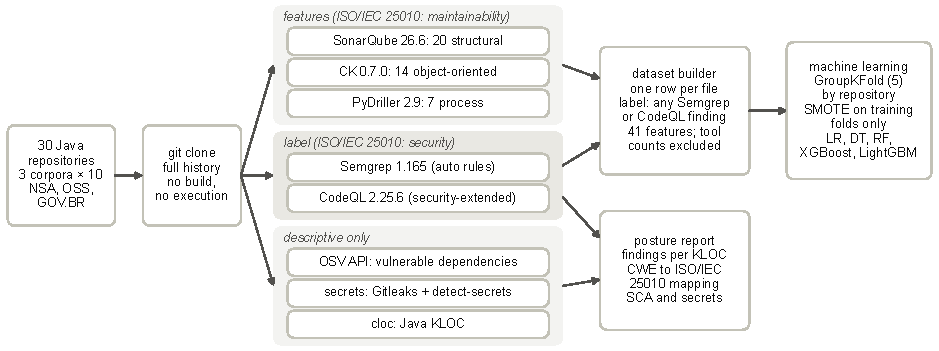
\includegraphics[width=\textwidth]{figures/fig_pipeline.pdf}
  \caption{The build-free pipeline. Repositories are cloned with their full history and never built; one tool per dimension produces the 41 features, the union of two SAST tools produces the label, and SCA, secret and size measures are descriptive only.}
  \label{fig:pipeline}
\end{figure*}

\subsection{Corpora}

We analyzed three corpora of ten public Java repositories each (Table~\ref{tab:corpora}). Repository selection was guided by five criteria, documented in the replication package: Java must dominate the code base, the repository must be publicly clonable, its history must be rich (at least 300 commits, five authors and two years), its size should lie roughly between 200 and 5,000 Java files, and it must contain genuine object-oriented code. Not every repository meets every criterion (for instance, Ghidra exceeds the size limit and four public-sector repositories share an organization); Section~\ref{sec:threats} discusses the consequences.

\textit{NSA.} Ten repositories of the NationalSecurityAgency GitHub organization: the reverse-engineering suite Ghidra, which alone holds 74.3\% of the Java code of the corpus, four repositories of the DataWave data-ingest ecosystem and five smaller projects. One organization and one dominant ecosystem make this corpus a confounded baseline.

\textit{OSS.} Ten projects with independent developer communities, one repository per project, covering network I/O (netty), authentication (shiro), service discovery (nacos), messaging (rocketmq), coordination (zookeeper), remote procedure calls (dubbo), continuous integration (jenkins), HTTP (httpcomponents-client), compression (commons-compress) and the Internet of Things (thingsboard). Six of them are Apache Software Foundation projects hosted under the same GitHub organization.

\textit{GOV.BR.} Ten repositories, taken from a predefined list of Brazilian public-sector systems and maintained by four organizations: the Demoiselle family (framework, signer, certificate and behave), IBICT (the institutional repositories \textit{deposita-dspace}, \textit{evidencia-dspace} and \textit{miguilim-dspace}, all based on DSpace, and a Dataverse instance), SIGA (document management) and LexML (legislative information services). The three DSpace-based repositories hold 66.3\% of the Java code. Table~\ref{tab:repos} lists the 30 repositories with their size, SAST findings and positive files.

\begin{table}[t]
\caption{Corpora, SAST findings and dataset composition. Largest repository: share of the Java KLOC held by the largest repository. Snapshot and history: .java files present in the analyzed snapshot and .java paths found only in the Git history, as shares of the dataset rows.}\label{tab:corpora}
\centering
\footnotesize
\begin{tabular}{@{}lrrr@{}}
\toprule
 & NSA & OSS & GOV.BR \\
\midrule
Repositories (orgs.) & 10 (1) & 10 (5) & 10 (4) \\
Java files & 21,254 & 25,506 & 13,635 \\
Java KLOC & 2,752 & 2,549 & 1,457 \\
Largest repository & 74.3\% & 20.9\% & 29.1\% \\
Semgrep findings & 575 & 1,230 & 2,193 \\
\quad in .java files & 39\% & 26\% & 20\% \\
CodeQL findings & 1,045 & 1,875 & 1,096 \\
OSV vuln. records & 56 & 7 & 469 \\
Candidate secrets & 564 & 3,805 & 627 \\
\midrule
Dataset rows & 31,622 & 64,415 & 33,521 \\
\quad .java, snapshot & 67.2\% & 39.8\% & 41.1\% \\
\quad .java, history & 27.4\% & 49.2\% & 43.4\% \\
\quad non-Java & 5.4\% & 11.0\% & 15.6\% \\
Positive rows & 560 & 839 & 784 \\
\quad positive rate & 1.77\% & 1.30\% & 2.34\% \\
\quad non-Java & 55 & 81 & 199 \\
\quad by both tools & 20 & 38 & 90 \\
CK coverage & 26.0\% & 96.8\% & 97.2\% \\
\bottomrule
\end{tabular}
\end{table}

\begin{table}[t]
\caption{Studied repositories: Java files, Java KLOC, SAST findings (Semgrep plus CodeQL) and positive dataset rows, ordered by size within each corpus.}\label{tab:repos}
\centering
\footnotesize
\setlength{\tabcolsep}{4pt}
\begin{tabular}{@{}lrrrr@{}}
\toprule
Repository & Files & KLOC & SAST & Pos. \\
\midrule
\multicolumn{5}{@{}l}{NSA} \\
ghidra & 15,589 & 2,046.2 & 616 & 253 \\
datawave & 4,302 & 565.9 & 707 & 221 \\
emissary & 676 & 67.4 & 124 & 45 \\
timely & 359 & 31.1 & 64 & 19 \\
datawave-query & 54 & 14.0 & 71 & 6 \\
lemongrenade & 110 & 13.9 & 5 & 3 \\
datawave-audit & 48 & 7.7 & 16 & 4 \\
datawave-authz & 51 & 3.5 & 10 & 6 \\
rank-based-linkage & 34 & 1.6 & 3 & 1 \\
fractalrabbit & 31 & 1.1 & 4 & 2 \\
\midrule
\multicolumn{5}{@{}l}{OSS} \\
nacos & 5,249 & 532.7 & 539 & 177 \\
netty & 3,589 & 430.0 & 966 & 143 \\
thingsboard & 4,780 & 406.7 & 452 & 167 \\
dubbo & 3,986 & 309.4 & 458 & 71 \\
rocketmq & 2,287 & 287.4 & 108 & 37 \\
jenkins & 1,946 & 208.5 & 269 & 110 \\
zookeeper & 943 & 126.7 & 103 & 50 \\
httpcomponents & 1,170 & 119.6 & 79 & 31 \\
commons-compress & 709 & 83.3 & 20 & 13 \\
shiro & 847 & 44.2 & 111 & 40 \\
\midrule
\multicolumn{5}{@{}l}{GOV.BR} \\
evidencia-dspace & 3,882 & 424.1 & 330 & 109 \\
deposita-dspace & 3,649 & 388.8 & 439 & 148 \\
siga & 2,104 & 225.5 & 1,475 & 180 \\
miguilim-dspace & 1,271 & 153.3 & 202 & 93 \\
dataverse & 959 & 147.8 & 631 & 166 \\
framework & 527 & 41.5 & 23 & 10 \\
behave & 515 & 34.7 & 75 & 33 \\
signer & 422 & 24.2 & 57 & 22 \\
certificate & 177 & 9.5 & 47 & 17 \\
eta-backend & 129 & 8.0 & 10 & 6 \\
\bottomrule
\end{tabular}
\end{table}

\subsection{A Build-Free Pipeline}

Figure~\ref{fig:pipeline} summarizes the pipeline. Repositories are cloned with their full history and are never built or executed, so the same procedure applies to any public Java repository, including projects whose builds depend on unavailable artifacts. The pipeline has 13 phases (clone, size, complexity, SonarQube, Semgrep, CodeQL, PyDriller, CK, OSV, secrets, dataset, machine learning and report), each implemented as an idempotent script whose failures are logged without aborting the run. A launcher redirects the input and output folders of each corpus, so the three corpora were processed by identical code.

We adopt one canonical tool per measurement dimension, because duplicated measures of the same construct introduce multicollinearity and blur feature-importance rankings. Structural measures come from SonarQube \cite{sonarqube}, run in source-only mode with the binaries property pointing to the sources (the lizard fallback for offline runs was not needed); object-oriented measures come from CK \cite{ck}; process measures come from PyDriller \cite{spadini2018}; dependencies declared in Maven and Gradle manifests are matched against OSV \cite{osv}; and secrets are the union of Gitleaks and detect-secrets findings, deduplicated by file, line and type \cite{gitleaks,detectsecrets}. Tool versions appear in Figure~\ref{fig:pipeline}.

\subsection{Security Label}

A file is labeled security-prone (positive) when at least one of two SAST tools reports a finding in it. Semgrep runs with its community auto configuration over the whole working tree \cite{semgrep}, and CodeQL runs the java-security-extended query suite on a database created with build mode none, that is, without compilation \cite{codeql}. We take the union because the tools are complementary and, in security, a missed weakness is the costlier error. The per-tool finding counts are kept for agreement analysis but are never used as features. SonarQube is not used as a security oracle, because its Java security rules need bytecode to fire.

\subsection{Features and Dataset}

Each file is described by 41 numeric features: 20 SonarQube measures (lines and non-comment lines of code, functions, classes, statements, cyclomatic and cognitive complexity, duplication, comments, code smells, technical-debt index and ratio, and rule-violation counts by severity), 14 CK measures aggregated from classes to files (WMC, RFC and the counts of methods, fields and classes are summed; DIT, NOC, CBO, LCOM, LCOM*, TCC and LCC take the maximum) and 7 PyDriller measures (commits, distinct authors, lines added and removed, churn, file age and days since the last change). All feature families relate to maintainability in ISO/IEC 25010, whereas the label relates to security; the study therefore asks whether measures of one characteristic predict weaknesses in the other.

The unit of analysis is the file. The dataset contains every file that appears in at least one feature table; the label is joined to this universe and missing measures are set to zero. Because SonarQube also indexes web and configuration files, and PyDriller reports files that no longer exist in the analyzed snapshot, the universe is broader than the current Java tree (Table~\ref{tab:corpora}). We keep this design as executed and quantify its effects in Section~\ref{sec:rq3}.

\subsection{Learning and Validation Protocol}

Algorithm~\ref{alg:protocol} summarizes the protocol. We use GroupKFold with five folds grouped by repository, so that no repository contributes files to both the training and the test set of a fold \cite{pedregosa2011}. Within each training fold, features are standardized for logistic regression only and the minority class is oversampled with SMOTE \cite{chawla2002}; the test fold keeps its natural class distribution. We compare logistic regression (LR), a decision tree (DT) with maximum depth 10, random forest (RF) \cite{breiman2001}, XGBoost \cite{chen2016} and LightGBM \cite{ke2017}, the ensembles with 200 estimators each; all models except XGBoost also use balanced class weights. Hyper-parameters, the random seed and the decision threshold (0.5) are fixed. Feature importance is the Gini importance of a random forest fitted to the whole dataset.

\begin{algorithm}[t]
 \caption{Labeling and evaluation protocol.}\label{alg:protocol}
 \KwData{collector outputs of one corpus}
 \KwResult{mean precision, recall, F1 and ROC-AUC per model}
 \ForEach{file $f$ in the union of the feature tables}{
   $y_f \leftarrow 1$ if Semgrep or CodeQL reports a finding in $f$, else $0$\;
   $x_f \leftarrow$ the 41 measures of $f$, missing values set to $0$\;
 }
 assign the repositories to five folds (GroupKFold)\;
 \ForEach{fold $k \in \{1,\dots,5\}$}{
   $T \leftarrow$ files of the other folds; $V \leftarrow$ files of fold $k$\;
   standardize $T$ and $V$ (logistic regression only)\;
   oversample the positives of $T$ with SMOTE\;
   \ForEach{model $m \in \{$LR, DT, RF, XGBoost, LightGBM$\}$}{
     fit $m$ on $T$; score $V$ with threshold $0.5$\;
   }
 }
 average every metric over the five folds\;
\end{algorithm}

GroupKFold assigns repositories to folds so as to balance fold sizes, so large repositories are tested alone. In GOV.BR, folds 1, 2 and 3 test \textit{evidencia-dspace}, \textit{siga} and \textit{deposita-dspace}, respectively; fold 4 tests \textit{signer}, \textit{certificate}, \textit{framework} and \textit{eta-backend-services}; and fold 5 tests \textit{behave}, \textit{dataverse} and \textit{miguilim-dspace}.

\subsection{Evaluation Metrics}

Let $\mathit{TP}$, $\mathit{FP}$ and $\mathit{FN}$ be the numbers of true positives, false positives and false negatives in a test fold. We report precision ($P$), recall ($R$) and their harmonic mean $F_1$,
\begin{equation}
P = \frac{\mathit{TP}}{\mathit{TP}+\mathit{FP}}, \qquad R = \frac{\mathit{TP}}{\mathit{TP}+\mathit{FN}},
\label{eq:pr}
\end{equation}
\begin{equation}
F_1 = \frac{2PR}{P+R},
\label{eq:f1}
\end{equation}
together with ROC-AUC, the area under the receiver operating characteristic curve, which equals the probability that a randomly chosen positive file receives a higher score than a randomly chosen negative file. ROC-AUC does not depend on the decision threshold and is insensitive to the base rate, whereas the measures of Equations~(\ref{eq:pr}) and~(\ref{eq:f1}) are computed at the default threshold and are directly affected by class imbalance: a random classifier has an expected ROC-AUC of 0.5 and an expected precision equal to the positive rate. Every metric is computed per fold and then averaged, so that folds of different sizes weigh equally.

% =====================================================================
\section{\uppercase{Results}}
\label{sec:results}
% =====================================================================

\subsection{RQ1: Security Posture across Corpora}

Table~\ref{tab:corpora} shows that GOV.BR, with the least Java code (1,457 KLOC, about half of each other corpus), produced the most SAST findings (3,289) and has the highest positive rate (2.34\%). Most of the difference comes from Semgrep, whose findings are dominated by files that are not Java: only 39\%, 26\% and 20\% of its findings in NSA, OSS and GOV.BR, respectively, are in \textit{.java} files. In OSS, 640 of the 1,230 findings are in YAML files, mostly continuous-integration workflows that reference mutable action tags and Docker Compose services that neither drop privileges nor use read-only file systems; in GOV.BR, 1,448 of the 2,193 findings are in HTML or XHTML pages. CodeQL, which analyzes the Java extraction (plus 49 XML files in GOV.BR), yields 0.38, 0.74 and 0.75 findings per KLOC.

\begin{figure*}[t]
  \centering
  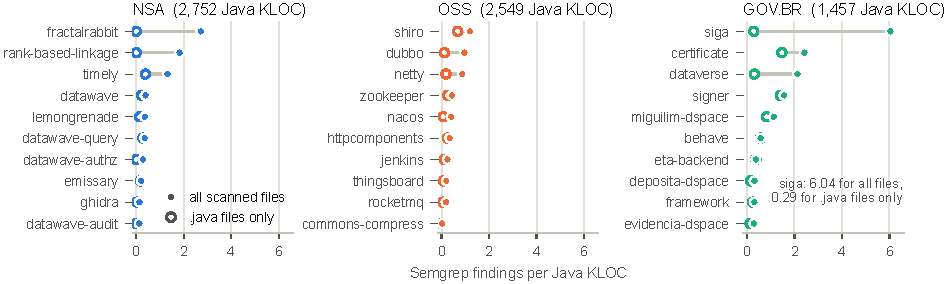
\includegraphics[width=\textwidth]{figures/fig_density.pdf}
  \caption{Semgrep findings per Java KLOC in each repository, counted over all scanned files (filled) and over .java files only (hollow). All panels share the same scale; the gap between the two markers is the contribution of web, configuration and vendored files.}
  \label{fig:density}
\end{figure*}

Figure~\ref{fig:density} normalizes Semgrep findings by Java KLOC. In NSA, the densest repositories are tiny research projects (\textit{fractalrabbit} has 1.1 KLOC and three findings), so their densities are unstable. In OSS, the three densest are libraries with an evident attack surface: \textit{shiro} (authentication), \textit{dubbo} (remote procedure calls and serialization) and \textit{netty} (network I/O). GOV.BR is dominated by \textit{siga}, whose 6.04 findings per KLOC are the highest of the 30 repositories. However, 1,072 of its 1,362 findings lie in a vendored copy of jQuery UI 1.10.3, 1,021 of them in the bundled HTML documentation of the library, and restricting the count to \textit{.java} files lowers its density to 0.29. Similarly, 210 of the 314 findings of \textit{dataverse} flag JSF pages that disable output escaping. Densities computed over all scanned files are therefore driven by third-party and non-Java artifacts.

The two SAST tools rarely agree. Among the positive files, only 20 of 560 (3.6\%) in NSA, 38 of 839 (4.5\%) in OSS and 90 of 784 (11.5\%) in GOV.BR are flagged by both tools, which supports the union as a recall-oriented label but also shows how strongly the label depends on the choice of tools. CodeQL alone flags most positives in NSA (349 of 560) and OSS (579 of 839) and 365 of the 784 positives in GOV.BR, where Semgrep findings in non-Java files account for another 178.

\begin{table}[t]
\caption{Most frequent CWEs of the Semgrep findings. The pipeline maps CWE-319 to confidentiality, maps CWE-470, CWE-79, CWE-89 and CWE-78 to integrity, and leaves the others unmapped.}\label{tab:cwe}
\centering
\footnotesize
\setlength{\tabcolsep}{4pt}
\begin{tabular}{@{}rlrrr@{}}
\toprule
CWE & Weakness & NSA & OSS & GOV.BR \\
\midrule
319 & Cleartext traffic & 104 & 117 & 1,148 \\
353 & No integrity check & 67 & 379 & 157 \\
1357 & Untrusted component & 50 & 358 & 86 \\
732 & Wrong permissions & 18 & 252 & 14 \\
470 & Unsafe reflection & 118 & 81 & 80 \\
150 & Improper escaping & 0 & 1 & 210 \\
79 & Cross-site scripting & 0 & 45 & 152 \\
89 & SQL injection & 99 & 26 & 36 \\
1333 & Inefficient regex & 9 & 83 & 47 \\
78 & Command injection & 43 & 15 & 2 \\
\bottomrule
\end{tabular}
\end{table}

Table~\ref{tab:cwe} lists the most frequent CWEs. In ISO/IEC 25010 terms, integrity weaknesses (mainly unsafe reflection and injection) dominate in NSA, unmapped configuration weaknesses in OSS, and cleartext transmission, a confidentiality weakness, in GOV.BR. Four weaknesses are among the six most frequent in every corpus: CWE-319 (cleartext transmission), CWE-470 (unsafe reflection), CWE-353 (missing integrity check) and CWE-1357 (reliance on insufficiently trustworthy components). The last two are not mapped by the pipeline and come mostly from configuration rather than Java code: the GitHub Actions rule on mutable action tags alone yields 50, 358 and 86 findings tagged with both CWEs, and HTML pages without subresource integrity account for the remaining CWE-353 findings. The profiles otherwise differ: NSA concentrates injection weaknesses (CWE-89 and CWE-78), OSS has permission problems in container configuration (CWE-732), and GOV.BR shows a web profile with cross-site scripting (CWE-79) and disabled escaping (CWE-150), besides 1,123 plaintext links in HTML pages that account for almost all of its CWE-319 findings.

Dependency analysis adds a different perspective. OSV matched 469 known-vulnerability records to the direct dependencies declared in GOV.BR, against 56 in NSA and 7 in OSS; \textit{miguilim-dspace} (154), \textit{siga} (142) and \textit{behave} (67) account for 77\% of them, which points to outdated dependencies rather than to weaknesses in the code itself. Secret scanning reported 564, 3,805 and 627 candidate secrets after deduplication, 2,247 of the OSS candidates in \textit{thingsboard} alone. Neither measure enters the models, but both inform the confidentiality and resistance sub-characteristics.

\begin{table}[t]
\caption{Static evidence per ISO/IEC 25010 security sub-characteristic: CWE tags of the Semgrep findings (a finding may carry several tags) and, for resistance, OSV vulnerability records of declared dependencies.}\label{tab:subchar}
\centering
\footnotesize
\begin{tabular}{@{}lrrr@{}}
\toprule
Sub-characteristic & NSA & OSS & GOV.BR \\
\midrule
Integrity & 278 & 179 & 372 \\
Confidentiality & 117 & 170 & 1,240 \\
Authenticity & 11 & 15 & 31 \\
Resistance (OSV) & 56 & 7 & 469 \\
Not mapped & 219 & 1,224 & 636 \\
\bottomrule
\end{tabular}
\end{table}

Table~\ref{tab:subchar} groups this evidence by security sub-characteristic. Integrity and confidentiality are the best covered, authenticity receives few findings (certificate validation and hard-coded credentials), and non-repudiation and accountability cannot be observed by static analysis at all. The large unmapped share of OSS reflects configuration weaknesses (CWE-353, CWE-1357 and CWE-732) that the pipeline's mapping does not assign to any sub-characteristic, although they arguably concern integrity and resistance; the mapping is thus a lower bound of the evidence available for the quality model.

\textit{Answer to RQ1.} GOV.BR has the weakest posture in SAST findings, positive rate and vulnerable dependencies, but in all corpora most Semgrep findings come from web pages, configuration files and vendored code rather than from the Java code that the features describe.

\subsection{RQ2: Predicting Security-Prone Files}

\begin{table*}[t]
\caption{Mean precision (P), recall (R), F1 and ROC-AUC over the five repository-grouped folds.}\label{tab:ml}
\centering
\footnotesize
\setlength{\tabcolsep}{4pt}
\begin{tabular}{@{}lrrrrcrrrrcrrrr@{}}
\toprule
 & \multicolumn{4}{c}{NSA} & & \multicolumn{4}{c}{OSS} & & \multicolumn{4}{c}{GOV.BR} \\
\cmidrule(lr){2-5}\cmidrule(lr){7-10}\cmidrule(lr){12-15}
Model & P & R & F1 & AUC & & P & R & F1 & AUC & & P & R & F1 & AUC \\
\midrule
Logistic regression & 0.089 & 0.705 & 0.158 & 0.815 & & 0.057 & 0.753 & 0.105 & 0.893 & & 0.096 & 0.751 & 0.162 & 0.854 \\
Decision tree & 0.145 & 0.426 & 0.213 & 0.762 & & 0.084 & 0.399 & 0.136 & 0.806 & & 0.170 & 0.553 & 0.255 & 0.804 \\
Random forest & 0.299 & 0.172 & 0.199 & 0.854 & & 0.175 & 0.098 & 0.117 & 0.891 & & 0.429 & 0.430 & 0.405 & 0.895 \\
XGBoost & 0.252 & 0.131 & 0.136 & 0.829 & & 0.161 & 0.062 & 0.086 & 0.862 & & 0.450 & 0.387 & 0.395 & 0.903 \\
LightGBM & 0.377 & 0.133 & 0.175 & 0.845 & & 0.177 & 0.062 & 0.089 & 0.872 & & 0.415 & 0.330 & 0.344 & 0.910 \\
\bottomrule
\end{tabular}
\end{table*}

Table~\ref{tab:ml} reports the mean performance of the five classifiers. All models rank SAST-flagged files well above chance in every corpus: ROC-AUC ranges from 0.762 (decision tree, NSA) to 0.910 (LightGBM, GOV.BR), and the tree ensembles exceed 0.82 everywhere. Precision, however, stays low because positives are rare. Logistic regression is the most stable model: its recall lies between 0.705 and 0.753 in the three corpora, at precisions between 0.057 and 0.096, that is, four to five times the base rate. In operational terms, inspecting the 16--21\% of the files that it flags would recover 70--75\% of the SAST-flagged files. The ensembles behave in the opposite way, trading recall (0.06--0.43) for precision (0.16--0.45). Results vary moderately across folds in NSA and OSS, where the standard deviation of the random-forest ROC-AUC over the five folds is 0.023 and 0.039, respectively, but the deviation reaches 0.110 in GOV.BR, a first sign that one of the corpora behaves differently.

GOV.BR stands out. Its ensembles combine the highest ROC-AUC with precision and recall between 0.33 and 0.45, and their F1 is more than three times that of the same models in OSS (0.405 versus 0.117 for random forest). A higher base rate makes positives easier to find, but it cannot explain a threefold gain, and the simplest model, logistic regression, does not share it. Section~\ref{sec:rq3} shows why.

\begin{table*}[t]
\caption{Random-forest Gini importance: share of each feature family (number of features in parentheses) and the five most important features of each corpus.}\label{tab:importance}
\centering
\footnotesize
\begin{tabular}{@{}llll@{}}
\toprule
 & NSA & OSS & GOV.BR \\
\midrule
SonarQube (20) & 68\% & 58\% & 74\% \\
CK (14) & 14\% & 28\% & 14\% \\
PyDriller (7) & 18\% & 14\% & 12\% \\
\midrule
1st & cognitive complexity (0.119) & cognitive complexity (0.113) & non-comment lines (0.104) \\
2nd & non-comment lines (0.082) & lines (0.085) & lines (0.103) \\
3rd & lines (0.064) & RFC (0.083) & rule violations (0.073) \\
4th & statements (0.059) & statements (0.080) & cognitive complexity (0.062) \\
5th & cyclomatic complexity (0.046) & non-comment lines (0.063) & technical-debt index (0.054) \\
\bottomrule
\end{tabular}
\end{table*}

Table~\ref{tab:importance} summarizes the random-forest importance. Structural measures carry 58--74\% of the importance in all corpora, object-oriented measures 14--28\% and process measures 12--18\%. Cognitive complexity is the most important feature in NSA and OSS, size (non-comment lines of code) in GOV.BR, and RFC is among the ten most important features in all three corpora; in OSS, where CK covers almost every file, RFC is the third most important feature. In ISO/IEC 25010 terms, the measures that predict the security label are maintainability measures of size and complexity. Part of this signal is plausibly mechanical, since larger and more complex files offer more locations for a finding.

\textit{Answer to RQ2.} Quality metrics rank SAST-flagged files consistently above chance (ROC-AUC 0.76--0.91), with size and complexity as the strongest predictors, but precision remains low; a high-recall linear model is the most stable option for triage.

\subsection{RQ3: Corpus Properties that Distort the Results}
\label{sec:rq3}

\begin{figure*}[t]
  \centering
  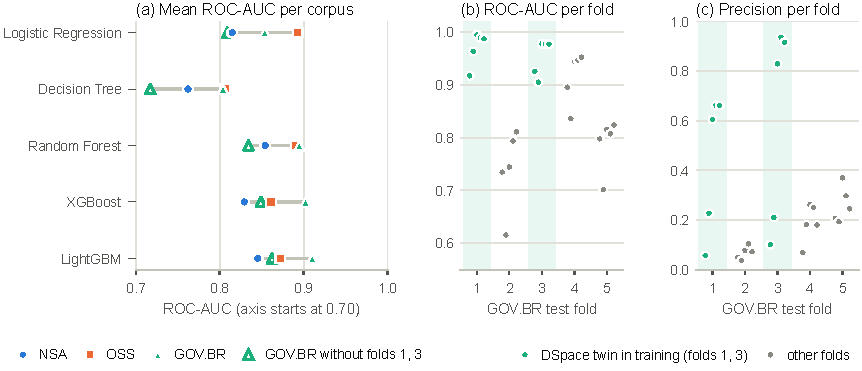
\includegraphics[width=\textwidth]{figures/fig_performance.pdf}
  \caption{(a) Mean ROC-AUC of each model in each corpus; the hollow triangle averages GOV.BR without folds 1 and 3. (b, c) ROC-AUC and precision of the five classifiers (one dot each) in every GOV.BR test fold. Folds 1 and 3 test evidencia-dspace and deposita-dspace, each while its near-duplicate twin is in the training set.}
  \label{fig:performance}
\end{figure*}

Figure~\ref{fig:performance}(b) and (c) break the GOV.BR results down by fold. In folds 1 and 3, every classifier exceeds 0.90 ROC-AUC and the three ensembles reach 0.977--0.994, with precision between 0.61 and 0.94. In the other folds, the same ensembles reach 0.74--0.95 ROC-AUC, and no classifier exceeds a precision of 0.37. Folds 1 and 3 test \textit{evidencia-dspace} and \textit{deposita-dspace}, two DSpace-based repositories that share most of their code. Hashing their working trees shows that 2,910 of the 3,652 Java files of \textit{deposita-dspace} (79.7\%) are byte-identical, at the same path, to files of \textit{evidencia-dspace}, and that 103 of the 109 positive files of \textit{evidencia-dspace} share their path with a positive file of \textit{deposita-dspace}. When one repository is tested, its twin is in the training set, and the models recognize files that they have already seen, with the same labels. The third DSpace-based repository, \textit{miguilim-dspace}, shares only 22 identical Java files (1.7\%) with the other two, and its fold (fold 5) shows no such effect.

\begin{table}[t]
\caption{Mean ROC-AUC and precision of each model in the GOV.BR folds whose DSpace twin is in the training set (folds 1 and 3) and in the remaining folds (2, 4 and 5).}\label{tab:folds}
\centering
\footnotesize
\begin{tabular}{@{}lrrrr@{}}
\toprule
 & \multicolumn{2}{c}{ROC-AUC} & \multicolumn{2}{c}{Precision} \\
\cmidrule(lr){2-3}\cmidrule(lr){4-5}
Model & 1, 3 & others & 1, 3 & others \\
\midrule
LR & 0.921 & 0.809 & 0.079 & 0.108 \\
DT & 0.934 & 0.718 & 0.219 & 0.137 \\
RF & 0.986 & 0.834 & 0.717 & 0.237 \\
XGBoost & 0.983 & 0.849 & 0.799 & 0.217 \\
LightGBM & 0.982 & 0.862 & 0.788 & 0.166 \\
\bottomrule
\end{tabular}
\end{table}

Table~\ref{tab:folds} compares the two groups of folds. Without folds 1 and 3, random forest averages 0.834 ROC-AUC and 0.237 precision, in line with NSA (0.854 and 0.299) and OSS (0.891 and 0.175), and Figure~\ref{fig:performance}(a) shows the same correction for every model. Logistic regression, whose linear decision boundary cannot memorize individual files, gains ROC-AUC but no precision in the DSpace folds (0.079 versus 0.108), whereas the precision of the tree ensembles triples or more. The best result of the study is therefore produced by leakage between near-duplicate repositories, not by a stronger signal in public-sector code. Grouping folds by repository is necessary but not sufficient: the grouping unit must be the code lineage, not the repository.

Three further properties of the corpora affect labels and features. First, non-Java files: 1,695, 7,104 and 5,222 dataset rows are not Java files, and 55, 81 and 199 positives (10\%, 10\% and 25\%) are web or configuration files, mostly flagged by Semgrep, whose labels Java-oriented measures can hardly explain. Second, historical files: 27\%, 49\% and 43\% of the rows are \textit{.java} paths that exist only in the Git history; they carry process measures but no structural ones and can never be positive, which makes part of the ranking task trivial and probably raises ROC-AUC. Third, missing measures: CK failed on Ghidra when it was run as a single batch, so object-oriented measures cover only 26\% of the Java files of NSA, against 97\% in the other corpora.

\textit{Answer to RQ3.} Near-duplicate forks inflate the GOV.BR results despite repository-grouped validation, and the inclusion of non-Java and historical files in the file universe weakens the link between features and labels in all corpora.

% =====================================================================
\section{\uppercase{Discussion}}
\label{sec:discussion}
% =====================================================================

\subsection{Implications}

\textit{For researchers.} Repository-grouped validation is a common safeguard in cross-project prediction, but it assumes that repositories are independent. Our GOV.BR corpus violates this assumption in a way that is hard to see in aggregate results: two of five folds carry the leak, and they raise the mean ROC-AUC of the random forest by only 0.06, a gain that is easily attributed to the domain. We recommend (i) deduplicating files by content hash across repositories before splitting, or grouping repositories that share code into the same fold; (ii) reporting fold-level results next to the means; (iii) restricting the file universe to the analyzed snapshot and the target language, or reporting such strata separately; and (iv) excluding vendored third-party code before running SAST. These recommendations echo earlier warnings about duplication in models of code \cite{allamanis2019,lopes2017} and about data snooping in security \cite{arp2022}; the novelty is that the leak appears even when the usual safeguard is in place.

\textit{For practitioners.} Quality metrics are not a substitute for SAST, but they can rank files when running and triaging SAST on every change is too expensive: in our corpora, a balanced logistic regression flags about one fifth of the files and recovers about three quarters of the SAST-flagged ones. For the public-sector systems, the posture data suggest concrete priorities: updating dependencies (469 vulnerability records concentrated in three repositories), enforcing output escaping in web templates, and removing vendored documentation and libraries from the source tree.

\textit{For the quality model.} The strongest predictors of the security label are maintainability measures of size and complexity, consistently with earlier metric-based studies \cite{shin2011,chowdhury2011,siavvas2020}. The dominance of size, however, suggests that part of the relation between the two ISO/IEC 25010 characteristics is a matter of opportunity: a larger file simply contains more code that a rule can match. Normalizing the label or the features by size is a natural next step before interpreting the relation causally.

\subsection{Lessons for Build-Free Pipelines}

Running the same code on three corpora exposed failure modes that a single run would hide. First, tools can fail silently: when CK processed Ghidra as a single batch, it produced no measures for any of its 15,589 Java files, and the graceful-degradation design of the pipeline turned the failure into zero-valued features instead of an error. Running CK per module root, as in the OSS and GOV.BR runs, raised its coverage to 97\%; per-tool coverage checks for every repository should be part of any such pipeline. Second, build-free analysis is feasible for Java: CodeQL extracted the Java code without compilation, and SonarQube produced structural measures in source-only mode, at the price of its security rules, which need bytecode. Third, scanning the whole working tree mixes languages and third-party code into the label; restricting SAST to first-party Java code, or stratifying the results by language, makes the label and the features describe the same artifacts. Fourth, running an unchanged pipeline on a new corpus is itself a validation step: the GOV.BR run reproduced the coverage obtained on OSS and revealed the fork effect, which a single-corpus study would not have exposed.

\subsection{Threats to Validity}
\label{sec:threats}

\textit{Construct validity.} The label is a proxy: SAST tools produce false positives and miss most real vulnerabilities \cite{li2023}, and our two tools agree on only 3.6--11.5\% of the positive files. Semgrep's community rules scan web and configuration files, so part of the label measures properties that the features do not describe. The CWE mapping leaves frequent weaknesses (e.g., CWE-353 and CWE-1357) unclassified, and non-repudiation and accountability cannot be measured statically. SonarQube's rule-violation counts are not split by issue type and may include the few security rules that run without bytecode; violations are among the most important features in GOV.BR, so a small amount of label leakage through this channel cannot be excluded. OSV records were counted, not weighted by severity.

\textit{Internal validity.} The file universe mixes current Java files with non-Java and historical files, and missing measures are set to zero; CK measures are missing for Ghidra. We used default hyper-parameters, a single seed and a fixed threshold, which may favor some models over others. The fork leak was diagnosed for the DSpace repositories; smaller near-duplicates may exist elsewhere and were not searched for systematically.

\textit{External validity.} The study covers 30 Java repositories in three corpora, two of which are dominated by a few code bases (Ghidra holds 74\% of the NSA code and the DSpace-based repositories 66\% of the GOV.BR code); six OSS projects belong to the Apache Software Foundation; and every corpus is a single snapshot. The results may not transfer to other languages, to proprietary code or to finer granularities such as methods.

\textit{Reliability.} The pipeline is static and versioned, its phases are idempotent, tool versions are fixed, and every phase stores its output as CSV files, so the analyses can be repeated without running the collectors again. Exact replication of the collection is nonetheless limited by evolving community rule sets and by the SonarQube server version.

% =====================================================================
\section{\uppercase{Conclusion}}
\label{sec:conclusion}
% =====================================================================

We applied one build-free pipeline, without changes, to three corpora of ten Java repositories each and asked whether code quality metrics predict files flagged by SAST tools. The security posture of the corpora differs mainly in artifacts that are not Java code: web pages, continuous-integration configuration and vendored libraries generate most of the Semgrep findings, and the public-sector corpus also has the largest number of known-vulnerable dependencies (RQ1). Quality metrics, dominated by size and complexity, rank SAST-flagged files consistently above chance, with ROC-AUC between 0.76 and 0.91, but precision stays low and a high-recall linear model is the most stable triage option (RQ2). The best result of the study, however, is an artifact: near-duplicate forks placed in different folds inflate ROC-AUC above 0.97 for the tree ensembles, and without the affected folds the public-sector corpus performs like the others (RQ3).

Future work will regroup the folds by code lineage using content hashes, restrict the file universe to the Java files of the analyzed snapshot, exclude vendored code before running SAST, adopt time-aware validation, and calibrate the SAST label against vulnerabilities confirmed in public advisories.

\section*{\uppercase{Acknowledgements}}

% TODO: review these statements before submission (and anonymize the URL for double-blind review).
% TODO: data_nsa/, data_govbr/ and reports_* are git-ignored today; commit them (and
%       Artigo_TCC/Real/scripts) before changing "will be made available" to "are available".
\begin{itemize}
  \item Conflicts of Interest: The authors have no conflicts of interest or competing interests to declare in the context of this paper.
  \item Financial and other Support: No funding was received for the work reported here.
  \item Data Sharing: The pipeline, the file-level datasets of the three corpora and the scripts that generate the figures will be made available at \url{https://github.com/IgorMariano25/AP2_PROJETO_SOFTWARE}.
  \item AI Tools: An AI assistant (Claude, Anthropic) was used to help draft and edit the text and to write the scripts that generate the figures; all numbers were recomputed from the pipeline outputs and checked by the authors.
\end{itemize}

\bibliographystyle{apalike}
{\small
\bibliography{references}}

\end{document}
